% Options for packages loaded elsewhere
\PassOptionsToPackage{unicode}{hyperref}
\PassOptionsToPackage{hyphens}{url}
%
\documentclass[
]{article}
\usepackage{lmodern}
\usepackage{amssymb,amsmath}
\usepackage{ifxetex,ifluatex}
\ifnum 0\ifxetex 1\fi\ifluatex 1\fi=0 % if pdftex
  \usepackage[T1]{fontenc}
  \usepackage[utf8]{inputenc}
  \usepackage{textcomp} % provide euro and other symbols
\else % if luatex or xetex
  \usepackage{unicode-math}
  \defaultfontfeatures{Scale=MatchLowercase}
  \defaultfontfeatures[\rmfamily]{Ligatures=TeX,Scale=1}
\fi
% Use upquote if available, for straight quotes in verbatim environments
\IfFileExists{upquote.sty}{\usepackage{upquote}}{}
\IfFileExists{microtype.sty}{% use microtype if available
  \usepackage[]{microtype}
  \UseMicrotypeSet[protrusion]{basicmath} % disable protrusion for tt fonts
}{}
\makeatletter
\@ifundefined{KOMAClassName}{% if non-KOMA class
  \IfFileExists{parskip.sty}{%
    \usepackage{parskip}
  }{% else
    \setlength{\parindent}{0pt}
    \setlength{\parskip}{6pt plus 2pt minus 1pt}}
}{% if KOMA class
  \KOMAoptions{parskip=half}}
\makeatother
\usepackage{xcolor}
\IfFileExists{xurl.sty}{\usepackage{xurl}}{} % add URL line breaks if available
\IfFileExists{bookmark.sty}{\usepackage{bookmark}}{\usepackage{hyperref}}
\hypersetup{
  pdftitle={Analysis of SARS-CoV-2 Sequencing Data from Experimentally Infected Hamsters and Ferrets},
  pdfauthor={Sara Tagol},
  hidelinks,
  pdfcreator={LaTeX via pandoc}}
\urlstyle{same} % disable monospaced font for URLs
\usepackage[margin=1in]{geometry}
\usepackage{longtable,booktabs}
% Correct order of tables after \paragraph or \subparagraph
\usepackage{etoolbox}
\makeatletter
\patchcmd\longtable{\par}{\if@noskipsec\mbox{}\fi\par}{}{}
\makeatother
% Allow footnotes in longtable head/foot
\IfFileExists{footnotehyper.sty}{\usepackage{footnotehyper}}{\usepackage{footnote}}
\makesavenoteenv{longtable}
\usepackage{graphicx,grffile}
\makeatletter
\def\maxwidth{\ifdim\Gin@nat@width>\linewidth\linewidth\else\Gin@nat@width\fi}
\def\maxheight{\ifdim\Gin@nat@height>\textheight\textheight\else\Gin@nat@height\fi}
\makeatother
% Scale images if necessary, so that they will not overflow the page
% margins by default, and it is still possible to overwrite the defaults
% using explicit options in \includegraphics[width, height, ...]{}
\setkeys{Gin}{width=\maxwidth,height=\maxheight,keepaspectratio}
% Set default figure placement to htbp
\makeatletter
\def\fps@figure{htbp}
\makeatother
\setlength{\emergencystretch}{3em} % prevent overfull lines
\providecommand{\tightlist}{%
  \setlength{\itemsep}{0pt}\setlength{\parskip}{0pt}}
\setcounter{secnumdepth}{-\maxdimen} % remove section numbering

\title{Analysis of SARS-CoV-2 Sequencing Data from Experimentally Infected
Hamsters and Ferrets}
\author{Sara Tagol}
\date{02 December, 2024}

\begin{document}
\maketitle

\hypertarget{background-and-overview}{%
\section{Background and Overview}\label{background-and-overview}}

This is a report on SARS-CoV-2, including some variant analysis (Koyama
\emph{et al.}, 2020). This report focuses on the analysis of SARS-CoV-2
sequencing data alongside tabular data, including a variant analysis and
data summary. The primary goal is to investigate patterns in viral
variants and correlate them with metadata such as geographic location.

Key objectives include: 1. Summarizing sequencing quality. 2.
Identifying frequent variants in the VCF files. 3. Correlating variant
frequency with metadata from the \texttt{SraRunTable}.

\hypertarget{methods}{%
\section{Methods}\label{methods}}

See the set of tutorials on the
\href{https://knausb.github.io/vcfR_documentation/index.html}{vcfR
package website}.

You may also want to use any of a range of different COVID data packages
and data sources:

\begin{itemize}
\tightlist
\item
  \url{https://kjhealy.github.io/covdata/}
\item
  \url{https://github.com/como-ph/oxcovid19}
\item
  \url{https://ropensci.org/blog/2020/10/20/searching-medrxivr-and-biorxiv-preprint-data/}
\item
  \url{https://covidtracking.com/data/api}

  \begin{itemize}
  \tightlist
  \item
    \texttt{readr::read\_csv("https://api.covidtracking.com/v1/states/daily.csv")}
  \end{itemize}
\end{itemize}

\hypertarget{sequencing-data-analysis}{%
\subsection{Sequencing Data Analysis}\label{sequencing-data-analysis}}

Sequencing data were processed using \texttt{bwa} for alignment and
\texttt{bcftools} for variant calling. The resulting VCF files were
analyzed for variant frequencies and annotated with metadata.

\hypertarget{tabular-data-analysis}{%
\subsection{Tabular Data Analysis}\label{tabular-data-analysis}}

The \texttt{SraRunTable.csv} was analyzed in R to summarize sample
metadata and investigate patterns by region and sequencing platform.

All analyses were conducted using R scripts integrated into this
RMarkdown file, ensuring reproducibility.

\hypertarget{results-and-discussion}{%
\section{Results and Discussion}\label{results-and-discussion}}

\hypertarget{figures}{%
\section{Figures}\label{figures}}

\begin{figure}
\centering
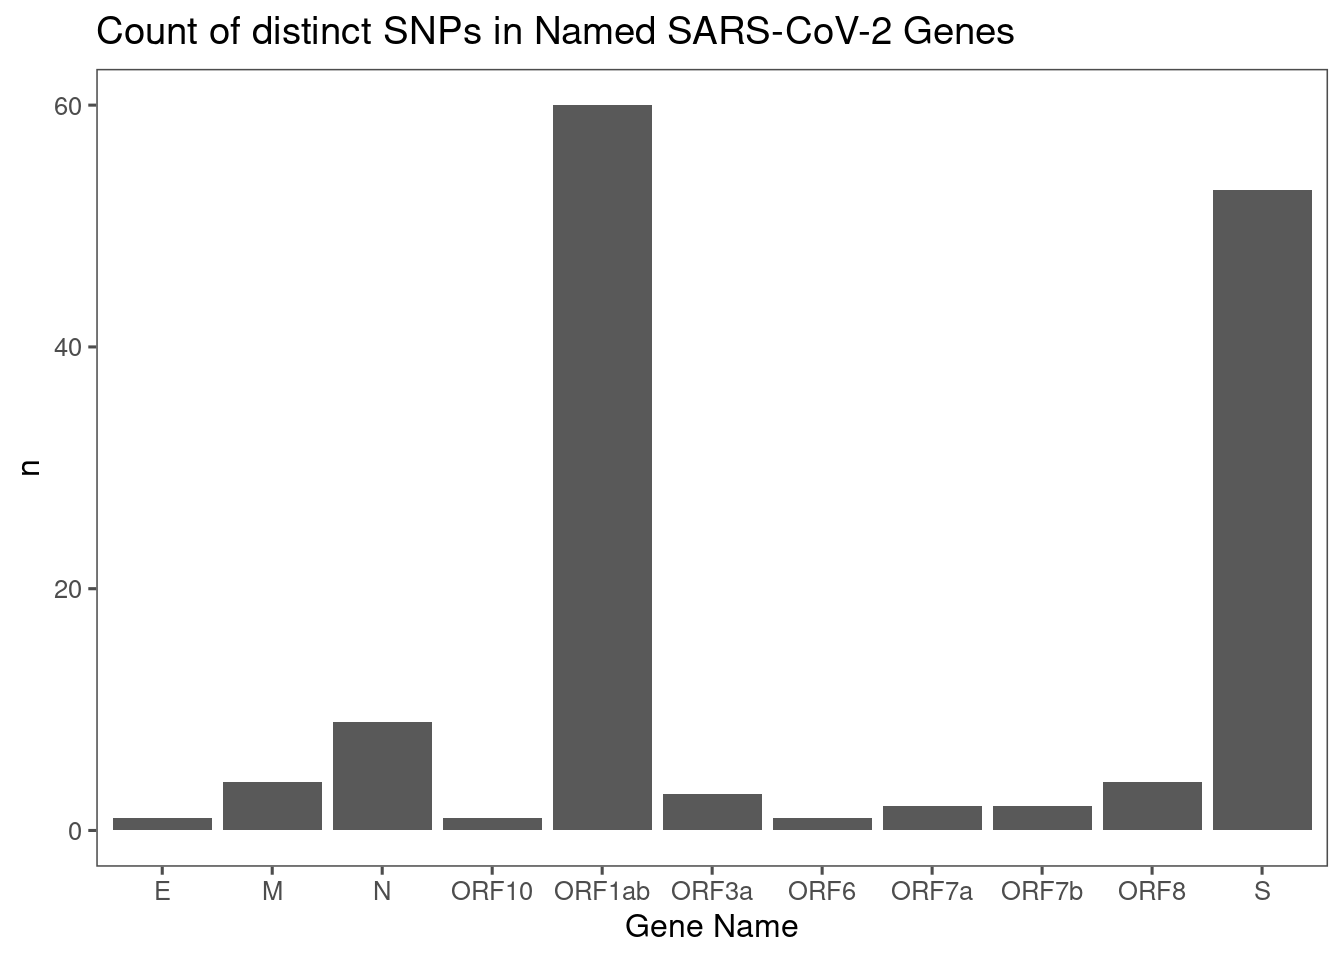
\includegraphics{Report_files/figure-latex/unique SNP locations-1.pdf}
\caption{Unique SNP Locations}
\end{figure}

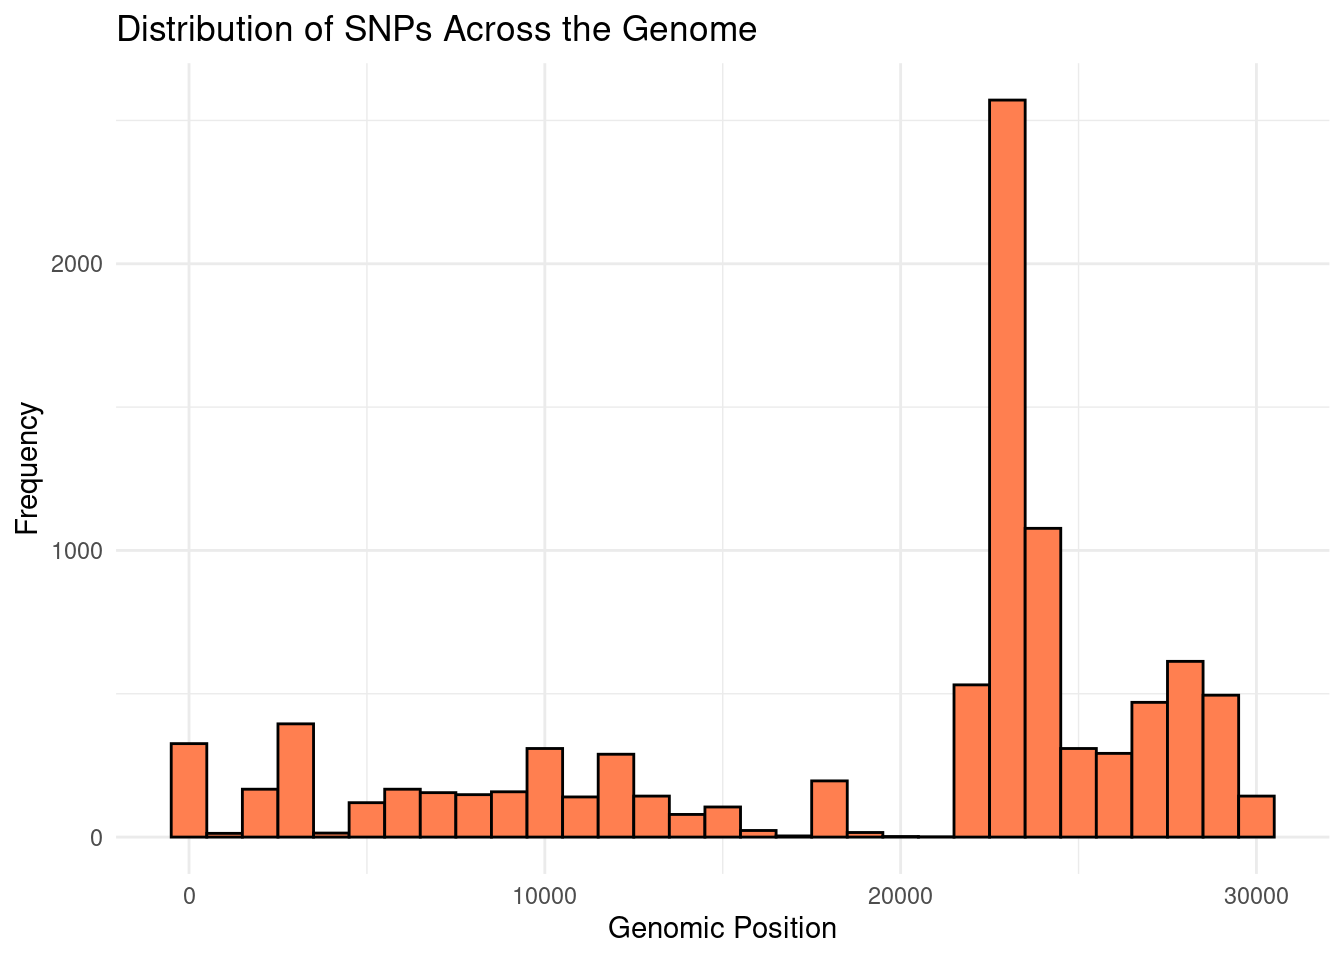
\includegraphics{Report_files/figure-latex/snp-distribution-genome-1.pdf}
\includegraphics{Report_files/figure-latex/ferret-hamster-sample-count-1.pdf}

\begin{figure}
\centering
\includegraphics{Report_files/figure-latex/snp-counts-sample-1.pdf}
\caption{SNP Counts Per Sample}
\end{figure}

\begin{figure}
\centering
\includegraphics{Report_files/figure-latex/gene-length-distribution-1.pdf}
\caption{Gene length distribution in SARS-CoV-2 genome}
\end{figure}

\begin{figure}
\centering
\includegraphics{Report_files/figure-latex/snp-gene-length-correlation-1.pdf}
\caption{Correlation between SNP counts and gene length}
\end{figure}

\textbf{Figure 1}: N and S genes have more unique SNPs in the set of
samples analyzed.

\hypertarget{tables}{%
\section{Tables}\label{tables}}

\begin{longtable}[]{@{}lrrr@{}}
\toprule
Gene Name & Start & End & Length\tabularnewline
\midrule
\endhead
ORF1ab & 266 & 21555 & 21289\tabularnewline
S & 21563 & 25384 & 3821\tabularnewline
ORF3a & 25393 & 26220 & 827\tabularnewline
E & 26245 & 26472 & 227\tabularnewline
M & 26523 & 27191 & 668\tabularnewline
ORF6 & 27202 & 27387 & 185\tabularnewline
ORF7a & 27394 & 27759 & 365\tabularnewline
ORF7b & 27756 & 27887 & 131\tabularnewline
ORF8 & 27894 & 28259 & 365\tabularnewline
N & 28274 & 29533 & 1259\tabularnewline
ORF10 & 29558 & 29674 & 116\tabularnewline
\bottomrule
\end{longtable}

\begin{longtable}[]{@{}lrrr@{}}
\toprule
Gene Name & Start & End & Length (bp)\tabularnewline
\midrule
\endhead
ORF1ab & 266 & 21555 & 21289\tabularnewline
S & 21563 & 25384 & 3821\tabularnewline
ORF3a & 25393 & 26220 & 827\tabularnewline
E & 26245 & 26472 & 227\tabularnewline
M & 26523 & 27191 & 668\tabularnewline
ORF6 & 27202 & 27387 & 185\tabularnewline
ORF7a & 27394 & 27759 & 365\tabularnewline
ORF7b & 27756 & 27887 & 131\tabularnewline
ORF8 & 27894 & 28259 & 365\tabularnewline
N & 28274 & 29533 & 1259\tabularnewline
ORF10 & 29558 & 29674 & 116\tabularnewline
\bottomrule
\end{longtable}

\begin{longtable}[]{@{}lr@{}}
\toprule
Gene Name & SNP Count\tabularnewline
\midrule
\endhead
S & 4473\tabularnewline
ORF1ab & 2645\tabularnewline
N & 654\tabularnewline
M & 376\tabularnewline
ORF3a & 168\tabularnewline
\bottomrule
\end{longtable}

\textbf{Table 1}: Gene names, locations, and lengths in the SARS-CoV-2
genome. Higher SNP counts in the S and N genes may be related to the
larger size of these genes.

\hypertarget{sources-cited}{%
\section*{Sources Cited}\label{sources-cited}}
\addcontentsline{toc}{section}{Sources Cited}

\hypertarget{refs}{}
\leavevmode\hypertarget{ref-koyama2020variant}{}%
Koyama,T. \emph{et al.} (2020) Variant analysis of sars-cov-2 genomes.
\emph{Bulletin of the World Health Organization}, \textbf{98}, 495.

\end{document}
